\section{Introduction}
\label{sec:intro}
\vspace{-1mm}

How do the brain and large language models represent emotions---and can their shared structure be exploited? Emotions in human psychology organize along continuous dimensions of valence and arousal~\cite{russell1980circumplex}, a geometry that neuroscience has shown is reflected in distributed neural representations. Recent interpretability research reveals a striking parallel: LLMs develop internal emotion representations with the same dimensional structure, emerging naturally from language modeling without explicit emotional supervision~\cite{sofroniew2026anthropic,tak2025emotion_interpretability,decoding_emotion_deep2024}. This convergence suggests a deep alignment between how biological and artificial neural networks encode affect---an alignment we propose to exploit for EEG-based emotion recognition. While EEG foundation models such as CBraMod~\cite{wang2025cbramod}, LaBraM~\cite{jiang2024labram}, and REVE~\cite{elouahidi2025reve} have established strong baselines on emotion benchmarks like FACED~\cite{chen2023faced}, they treat emotion categories as integer indices, discarding the relational structure that both brains and LLMs naturally encode.

The standard cross-entropy loss penalizes all misclassifications equally---confusing \emph{joy} with \emph{amusement} costs the same as confusing \emph{joy} with \emph{anger}. Recent work has begun to address this: EmotionCLIP~\cite{emotionclip2025} reformulates EEG emotion recognition as EEG-text matching using CLIP embeddings of emotion labels, while EMOD~\cite{emod2026} projects labels into a continuous valence--arousal space with soft-weighted contrastive learning. However, these approaches rely on hand-crafted text templates or predefined coordinate systems. We propose instead to use the \emph{internal} emotion geometry that emerges within LLMs---a richer, data-driven representation that encodes not just valence--arousal position but the full relational structure among emotions, including within-valence distinctions (e.g., \emph{anger} vs.\ \emph{fear} vs.\ \emph{disgust}).

\begin{wrapfigure}{r}{0.5\textwidth}
\vspace{-4mm}
\vspace{-\intextsep}
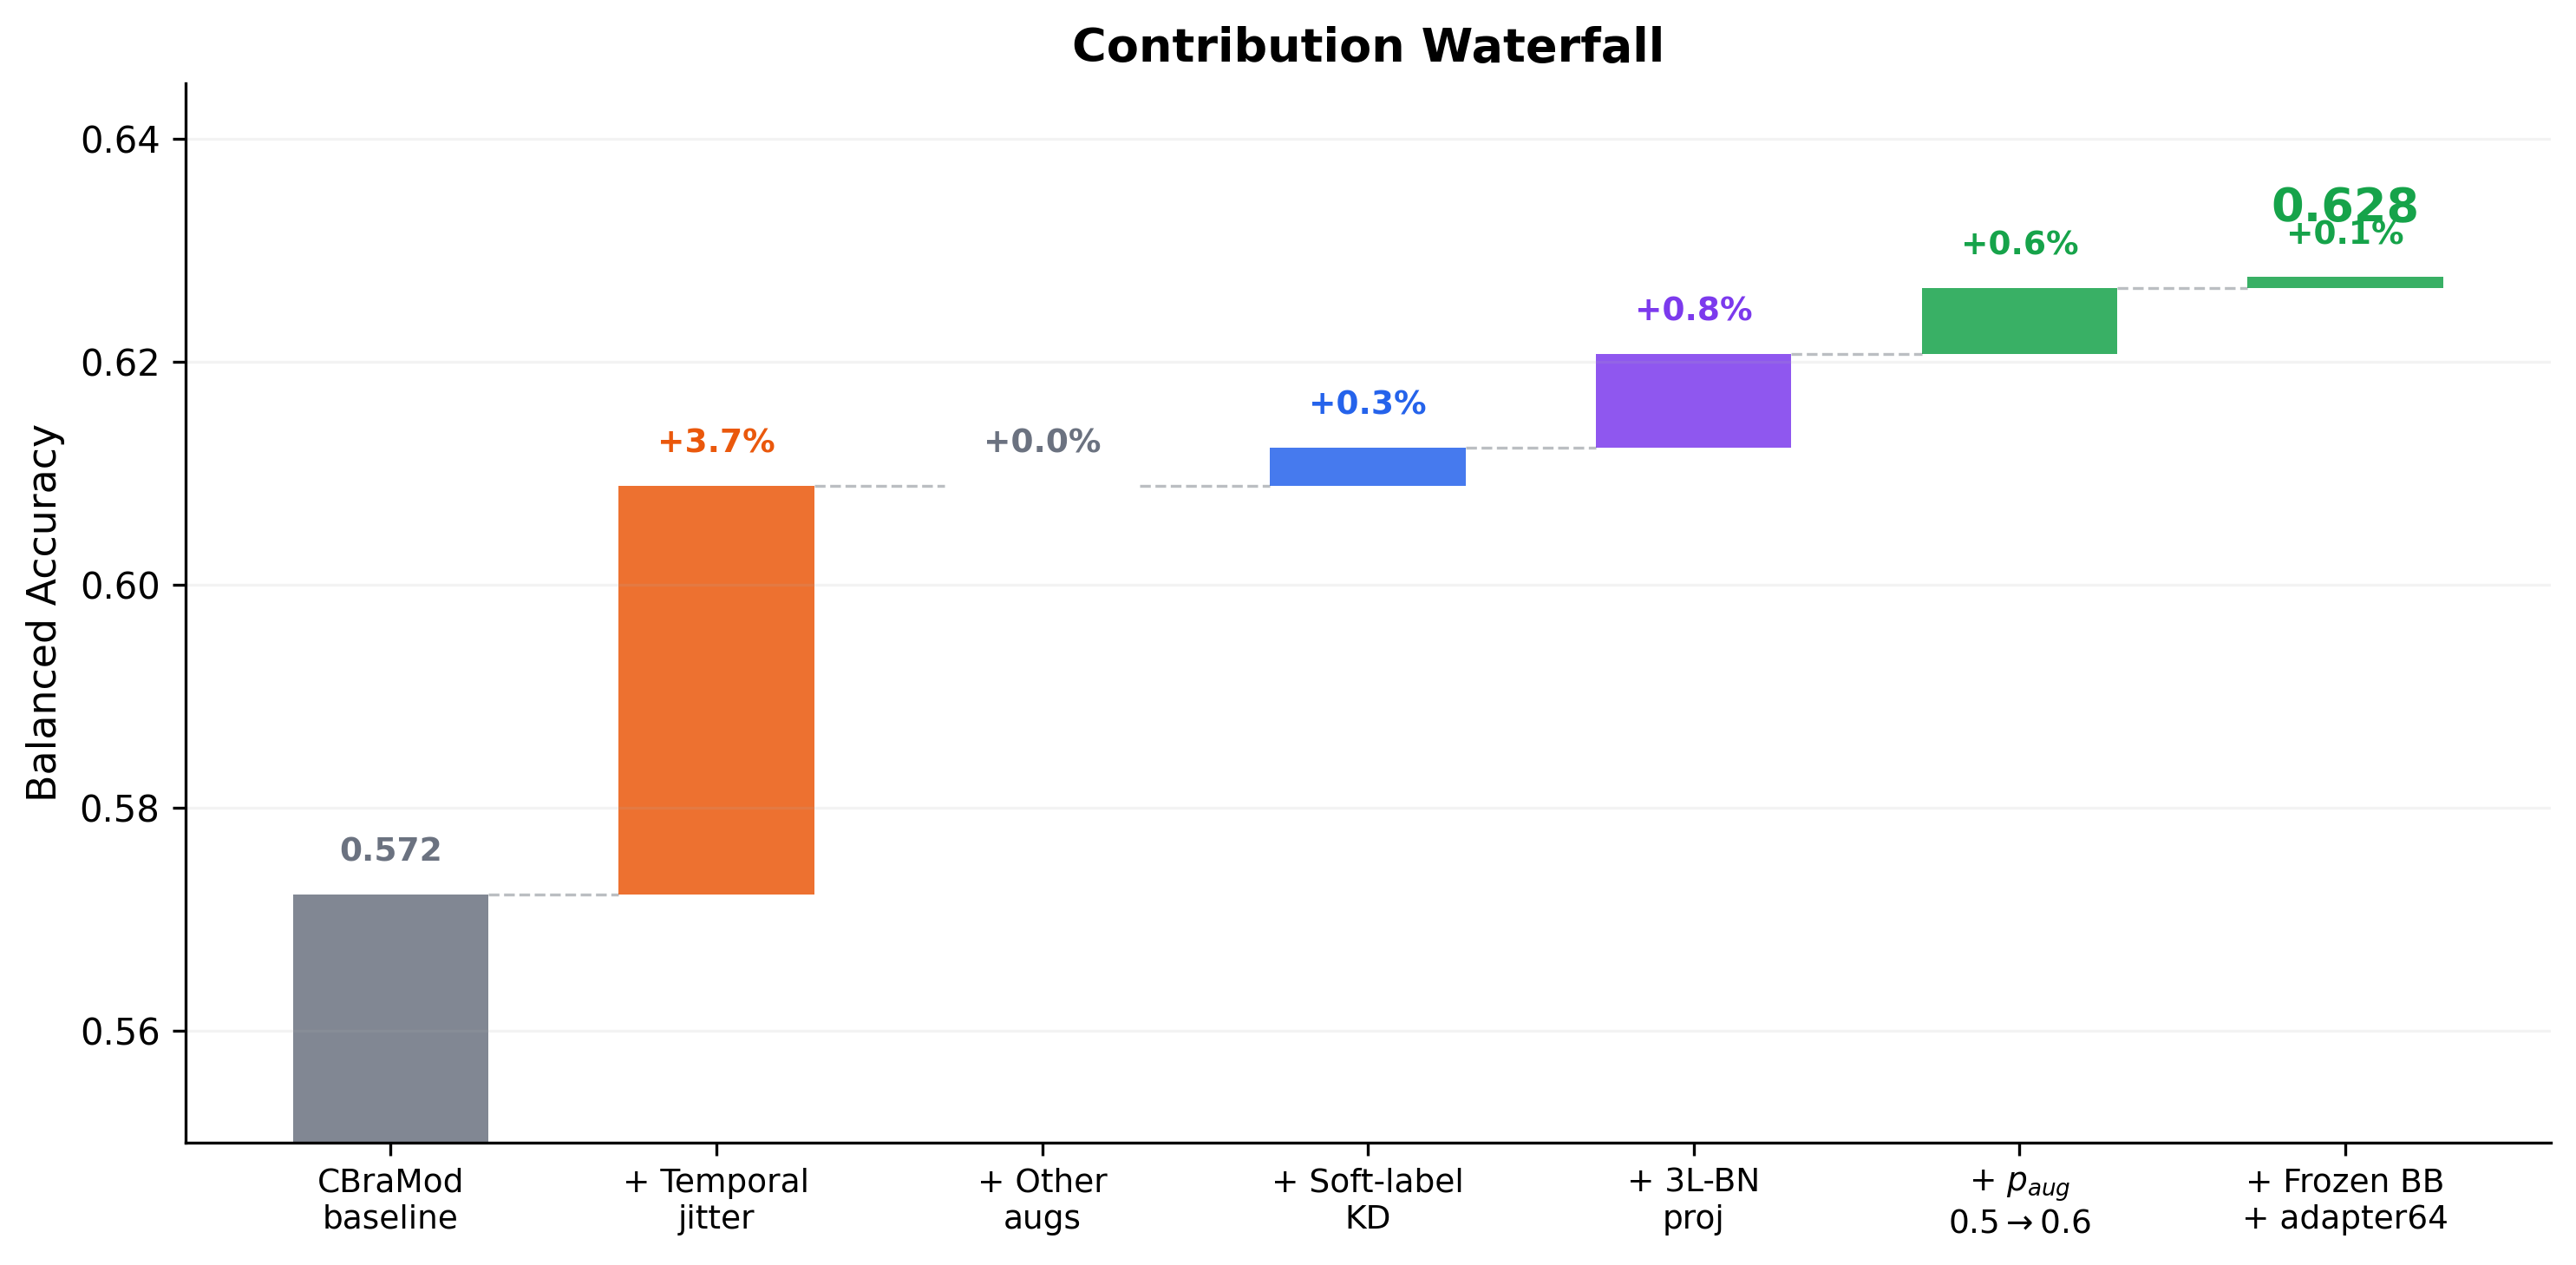
\includegraphics[width=\linewidth]{figs/waterfall.png}
\captionsetup{
  width=\linewidth,
  justification=raggedright,
  singlelinecheck=false
}
\caption{Contribution of each component of \ours\ to the final performance on FACED 9-class emotion recognition. KD adds $+1.8\%$ over augmentation alone; adapter PEFT preserves the gain with $20\times$ fewer trainable backbone parameters.}
\label{fig:teaser}
\end{wrapfigure}

We introduce \ours, a method that bridges LLM emotion representations and EEG through soft-label knowledge distillation. Given any instruction-tuned LLM, we extract emotion vectors by prompting the model to generate emotion-laden stories and recording hidden state activations at intermediate layers. These vectors define a similarity matrix that serves as soft targets for a KL-divergence-based KD loss, replacing the standard integer-label cross-entropy with a distribution that encodes \emph{how similar} each pair of emotions is. We combine this with temporal jitter augmentation---which we show through ablation is the single critical augmentation for EEG emotion classification---and a 3-layer BatchNorm projection head inspired by SimCLR v2~\cite{simclr_v2}.

\textbf{Three orthogonal axes of validation.} A core methodological contribution of this paper is to evaluate the framework along three independent axes:
\textbf{(1) Cross-backbone:} we replicate KD on both CBraMod (criss-cross transformer, ICLR 2025) and LaBraM (standard ViT, ICLR 2024) and find significant improvements on both ($+5.2\%$ and $+2.6\%$).
\textbf{(2) Cross-dataset:} we test on FACED (9 classes) and SEED-V (5 classes), where the KD effect on SEED-V is unlocked when input granularity is increased to 5\,s windows ($+1.85\%$ on LaBraM, $p = 0.037$). This reveals a practical \emph{token-count requirement}: KD efficacy scales monotonically with the number of EEG tokens per sample.
\textbf{(3) Cross-LLM-family:} we extract emotion vectors from 11 instruction-tuned models in two families (7 Qwen2.5 sizes + 4 Gemma-4 variants), and find that within-family and cross-family RDM agreement are nearly identical (within $\rho \approx 0.89$, cross $\rho = 0.82$), confirming that LLM emotion geometry is genuinely universal across families.

A second key finding emerges from our representational alignment analysis: \textbf{Centered Kernel Alignment (CKA)}~\cite{kornblith2019cka} between LLM features and EEG features increases for \emph{every} LLM in our 11-model suite after KD ($\Delta$CKA $\approx +0.03$), and the highest post-KD alignment is achieved with Gemma-4 31B---even though training used Qwen-14B as the teacher. This argues that KD does not simply pull EEG features toward the specific teacher; it absorbs a universal emotion structure that aligns with all sufficiently capable instruction-tuned LLMs.

We additionally find that \textbf{freezing the pretrained CBraMod backbone and adding lightweight bottleneck adapters (310K trainable parameters) matches full fine-tuning} on FACED, achieving balanced accuracy $\mathbf{0.628}$. This suggests that pretrained EEG representations already contain the information needed for emotion classification; the critical factor is the \emph{quality of the supervision signal} (LLM-guided KD), not the number of parameters being updated. We validate this finding through a systematic sweep of adapter bottleneck dimensions, showing a clear scaling curve with an optimal capacity at rank 64.

We evaluate \ours\ across two benchmark datasets in both within-subject and cross-subject settings:
\textbf{(1) FACED} (9-class, 123 subjects, 32 channels): balanced accuracy \(\mathbf{0.628}\), improving over the previous SOTA (REVE, NeurIPS 2025) by \(\mathbf{+11.2\%}\) relative.
\textbf{(2) SEED-V} (5-class, 16 subjects, 62 channels): with the 5\,s preprocessing variant, KD significantly improves balanced accuracy and Cohen's $\kappa$ on both backbones, with bootstrap 95\% confidence intervals that exclude zero.
Cross-subject evaluation on FACED (5-fold leave-group-out) shows significant improvement over baseline ($p < 0.001$), confirming generalization to unseen subjects.

In summary, the contributions of this paper include:
(1) \textbf{A novel knowledge distillation framework} that uses LLM-internal emotion representations as soft supervision targets for EEG emotion classification, outperforming standard contrastive alternatives (SupCon, valence--arousal coordinates) by $+1.8\%$.
(2) \textbf{Cross-backbone, cross-dataset, and cross-LLM-family validation}---the most thorough validation of an EEG-LLM alignment framework to date.
(3) \textbf{Empirical CKA evidence} that KD increases representational alignment between EEG and \emph{every} instruction-tuned LLM (not just the training teacher), indicating that KD absorbs a universal emotion structure.
(4) \textbf{The frozen-backbone + adapter finding}, showing that the quality of LLM-guided supervision matters more than trainable parameter count.
(5) \textbf{Analysis of LLM emotion geometry universality} across 11 instruction-tuned models from 2 families (Qwen2.5 0.5B--72B and Gemma-4 E2B--31B), with detailed scale analysis and a token-count guideline for applying KD to compressed EEG representations.
(6) \textbf{Manifold quality analysis} showing KD improves cluster separation by 38\% (Davies-Bouldin) and doubles the number of valence-correlated principal components, with a practical payoff: $+5.7\%$ at 1-shot cross-subject calibration.
(7) \textbf{Feature editability analysis} demonstrating that trained EEG features support data-driven emotion steering via contrastive activation addition~\cite{rimsky2024steering}, with KD creating a more structured and interpretable emotion manifold than baseline training.
